\chapter{Methodology} \label{ch:methodology}

In this chapter, our \acrshort{wsol} evaluation methodology is explained in detail. We start by describing the general approach for CAM-based localization in the end-to-end setup. This approach serves as a blueprint for the different localization techniques used. Next we specify the different networks and datasets used to train and evaluate models. Subsequently, the training process if defined. In the penultimate section, each localization method is discussed in detail. Finally we explain how we investigate localization improvements for multiple-instance localization.

\section{Networks}
The \acrshort{cam}-based \acrshort{wsol} methods require a \acrshort{cnn} model to classify images and localize objects in those images. We use the VGG16 and Resnet50 network. VGG16 and a variant of it for \acrshort{cam} is used in a lot of \acrshort{cam}-based papers and a good reference for benchmarking \acrshort{wsol}. Resnet50 is more recent and is used for experiments with MinMaxCAM by Wang, Kaili \textit{et al.}

\subsection{VGG16}
VGG16 is a \acrshort{cnn} proposed by K. Simonyan \textit{et al.} \cite{simonyan2014very}. It is one of the most popular models for image classification and it achieves high test accuracy for ImageNet, which is a very large dataset with 1000 different classes.
\begin{figure}[ht]
    \begin{center}       
    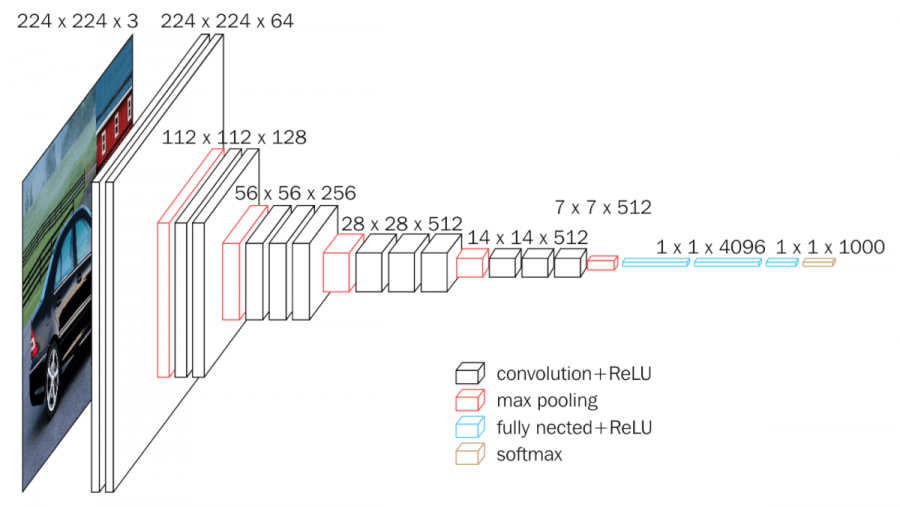
\includegraphics[width=1.0\textwidth]{fig_vgg16_arch.png}
    \caption[VGG16 architecture]{VGG16 architecture.}
    \caption*{Source: \href{https://neurohive.io/en/popular-networks/vgg16}{https://neurohive.io/en/popular-networks/vgg16}}
    \label{fig:vgg16_arch}
    \end{center}
\end{figure}

The VGG16 network architecture is shown in Fig. \ref{fig:vgg16_arch}. The 16 in VGG16 refers to 16 layers that have trainable weights. In VGG16 there are thirteen convolutional layers, five maximum pooling layers, and three dense layers. Each layer in the network is tagged with the dimensions of its output a color that represents its function. Fig. \ref{fig:vgg16_layers_auth} tags the network layers with unique names that we will use to refer to those layers. Convolutional layers are organized in blocks. Layers within a block have the same number of filters.
\begin{figure}[ht]
    \begin{center}       
    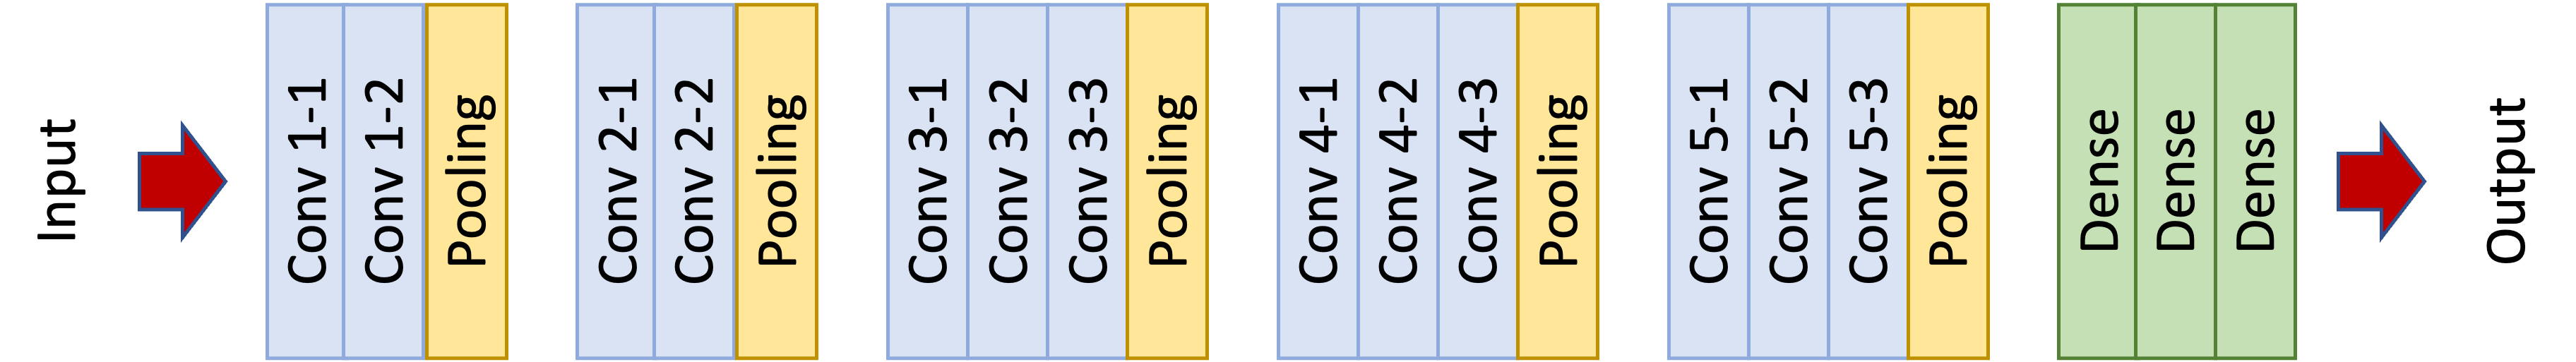
\includegraphics[width=1.0\textwidth]{fig_vgg16_layers_auth.png}
    \caption[VGG16 network layers]{VGG16 network layers.}
    \caption*{Source: Author}
    \label{fig:vgg16_layers_auth}
    \end{center}
\end{figure}

In subsequent sections, we describe the different parts of the architecture.
\subsubsection{Input}
The model expects as input images of fixed size and number of color channels. The dimensions are 224×224x3, standing for width x height x color channels. Typically images in popular datasets (e.g., Imagenet) have different sizes, requiring transformation of the images to resize them to the expected input shape.

\subsubsection{Convolutional layers}
The convolutional layers use a small kernel size of 3×3. A smaller kernel reduces the network’s tendency to over-fit during training. Conv-1 has 2 layers with 64 filters, Conv-2 has 2 layers with 128 filters, Conv-3 has 3 layers with 256 filters, Conv 4 and Conv 5 each have 3 layers with 512 filters. The number of filters represent the output channels of each layer.

\subsubsection{Activation function}
Each convolutional layer is followed by a \acrfull{relu} component. This activation function is a linear function that provides a matching output for positive inputs and outputs zero for negative inputs. The \acrshort{relu} function overcomes the vanishing gradient problem, allowing models to learn faster and perform better. Vanishing gradients occur when more and more layers are used. In this case the gradient can be too small for training to work effectively.

\subsubsection{Pooling layers}
A pooling layer follows a block of convolutional layers with the same kernel size. Pooling helps to reduce the size of the feature maps created by each convolution step. Pooling is given the increase  of the number of filters when going deeper in the network. When the number of filters doubles, also the number of feature maps doubles. The pooling window of 2x2 reduces the size of feature maps by four, keeping computational complexity balanced as we go deeper in the network.

\subsubsection{Fully connected layers}
Three \acrshort{fc} layers follow a stack of convolutional layers: The first two have 4096 channels each, the third performs 1000-way  classification and thus contains 1000 units (one for each class). The final layer is the soft-max layer. This layer ensures that the output values are transformed into confidence scores: Each output value is between 0 and 1 and the total sum of all outputs is 1.

Due to its depth and number of fully-connected nodes, VGG16 has 138 million weights with a storage size over 533MB. This puts high computational and storage requirements on training and storing a model.

\subsection{VGG16-GAP}
Zhou \textit{et al.} \cite{zhou2016cvpr} found that convolutional units to localize objects despite being trained on image-level labels. Despite this fact, this ability is lost when fully-connected layers are used for classification. Zhou \textit{et al.} found that by adding a \acrshort{gap} and tweaking the network, the localization ability of a \acrshort{cnn} can be kept until the final convolutional layer. We refer to this tweaked version of a VGG16 network as the VGG16-GAP network.

Zhou \textit{et al.} found that the localization ability of the network improved when the last convolutional layer before \acrshort{gap} has a higher spatial resolution. Therefore VGG16 is tweaked as illustrated in Fig. \ref{fig:vgg16_gap_layers_auth}. The pooling layer and \acrshort{fc} layers after Conv-5 are removed, resulting in a feature map with resolution 14x14. Then a convolutional layer Conv6-1 is added with kernel size 3×3 and 1024 units, followed by a GAP layer and a \acrshort{fc} and softmax layer.
\begin{figure}[ht]
    \begin{center}       
    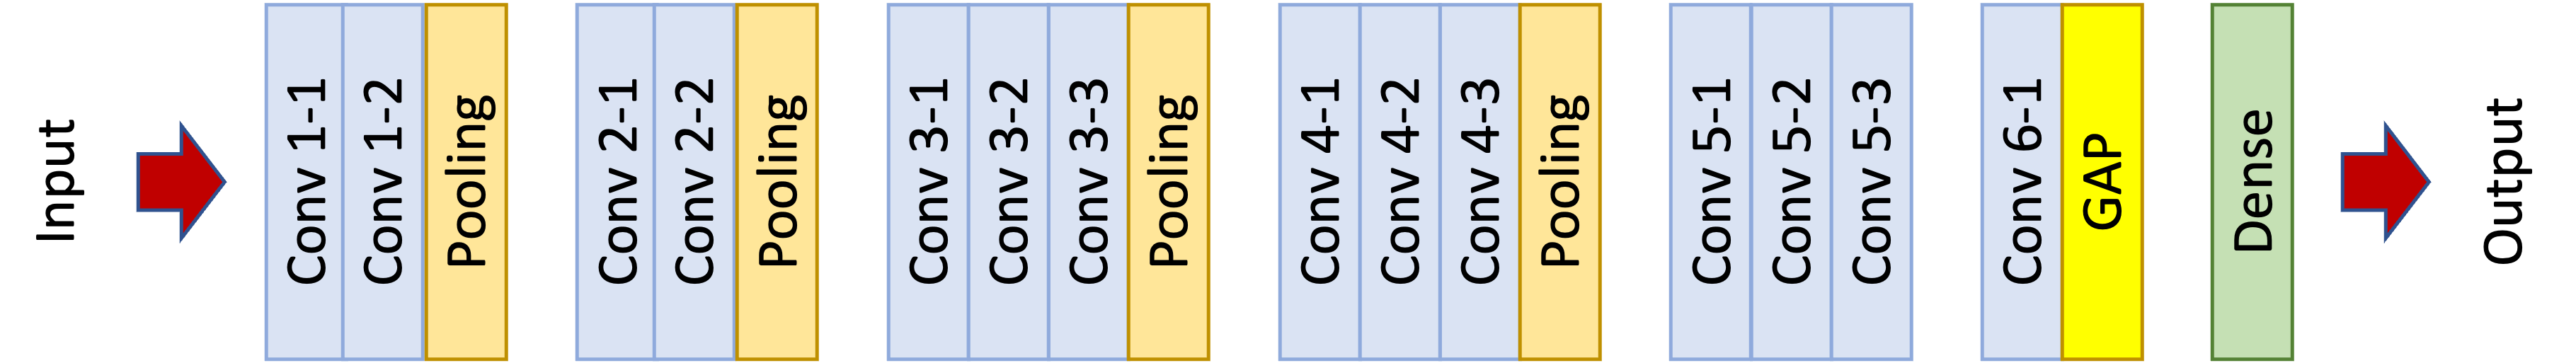
\includegraphics[width=1.0\textwidth]{fig_vgg16_gap_layers_auth.png}
    \caption[VGG16-GAP network layers]{VGG16-GAP network layers.}
    \caption*{Source: Author}
    \label{fig:vgg16_gap_layers_auth}
    \end{center}
\end{figure}

Note that removing fully-connected layers largely decreases network parameters, but also brings some classification performance drop. VGG16-GAP las 20 million parameters.

%picture, how it is used and modified for CAM method localization
%parameter count

\subsection{ResNet50 network}
% resaon: Used in MinMaxCAM, more recent than VGG16, efficient (skip 
% explain architecture: deeper networks using skip connections with less parameters connections)
Network depth is of crucial importance in neural network architectures, but deeper networks are more difficult to train. The residual learning framework eases the training of these networks, and enables them to be substantially deeper — leading to improved performance in both visual and non-visual tasks. These residual networks are much deeper than their ‘plain’ counterparts, yet they require a similar number of parameters (weights).

VGG introduced the concept of increasing the number of layers to improve accuracy. However, deeper networks are more difficult to train. He \textit{et al.} \cite{he2016deep} states that with network depth increasing, accuracy gets saturated and then degrades rapidly. This degradation leads to higher training error. The authors propose a solution to a deeper network that by construction should not have a higher training error than more shallow networks: The layers are copied from a learned shallower model and added layers are an identity mapping. The basic building block of residual networks is shown in Fig. \ref{fig:resnet_block}. The original non-residual mapping is cast into a residual mapping, that should be easier to optimize. This basic building block is used in residual networks with 18 or 34 trainable layers. 
\begin{figure}[ht]
    \begin{center}       
    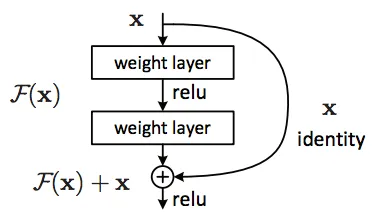
\includegraphics[width=0.4\textwidth]{fig_resnet_block.png}
    \caption[Residual block]{A residual. The fundamental building block of residual networks.}
    \caption*{Source: \href{https://medium.com/@waya.ai/deep-residual-learning-9610bb62c355}{https://medium.com/@waya.ai/deep-residual-learning-9610bb62c355}}
    \label{fig:resnet_block}
    \end{center}
\end{figure}

For deeper residual networks there is a concern on training time. Therefore, the basic building block is modified using a bottleneck design. An example is shown in Fig. \ref{fig:resnet_bottleneck}. For each residual function, a stack of three layers is used instead of two. The three layers are 1x1, 3x3, and 1x1 convolutions, where the 1x1 layers
are responsible for reducing and then increasing dimensions, leaving the 3x3 layer a bottleneck with smaller input/output dimension. For Resnet50, all basic building blocks from Resnet34 are replaced with bottleneck blocks, yielding 50 layers with learnable weights.
\begin{figure}[ht]
    \begin{center}       
    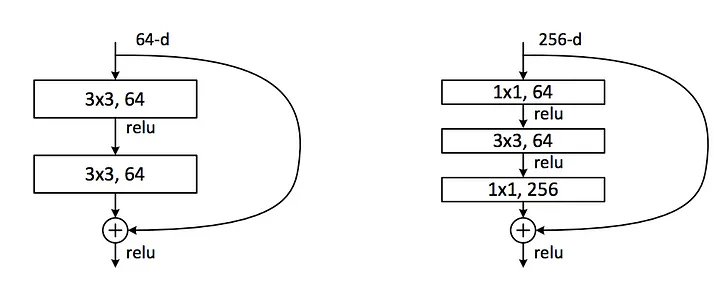
\includegraphics[width=0.7\textwidth]{fig_resnet_bottleneck.png}
    \caption[Residual basic and bottleneck blocks]{Basic residual block (left) and bottleneck residual block (right). Both designs have similar time complexity.}
    \caption*{Source: \href{https://medium.com/@waya.ai/deep-residual-learning-9610bb62c355}{https://medium.com/@waya.ai/deep-residual-learning-9610bb62c355}}
    \label{fig:resnet_bottleneck}
    \end{center}
\end{figure}

The detailed architecture of ResNet50 and other variants are shown in Fig. \ref{fig:resnet_arch_table}. Although resnet50 has many more layers than VGG16, it has 25 million parameters which is far less than VGG16. 
\begin{figure}[ht]
    \begin{center}       
    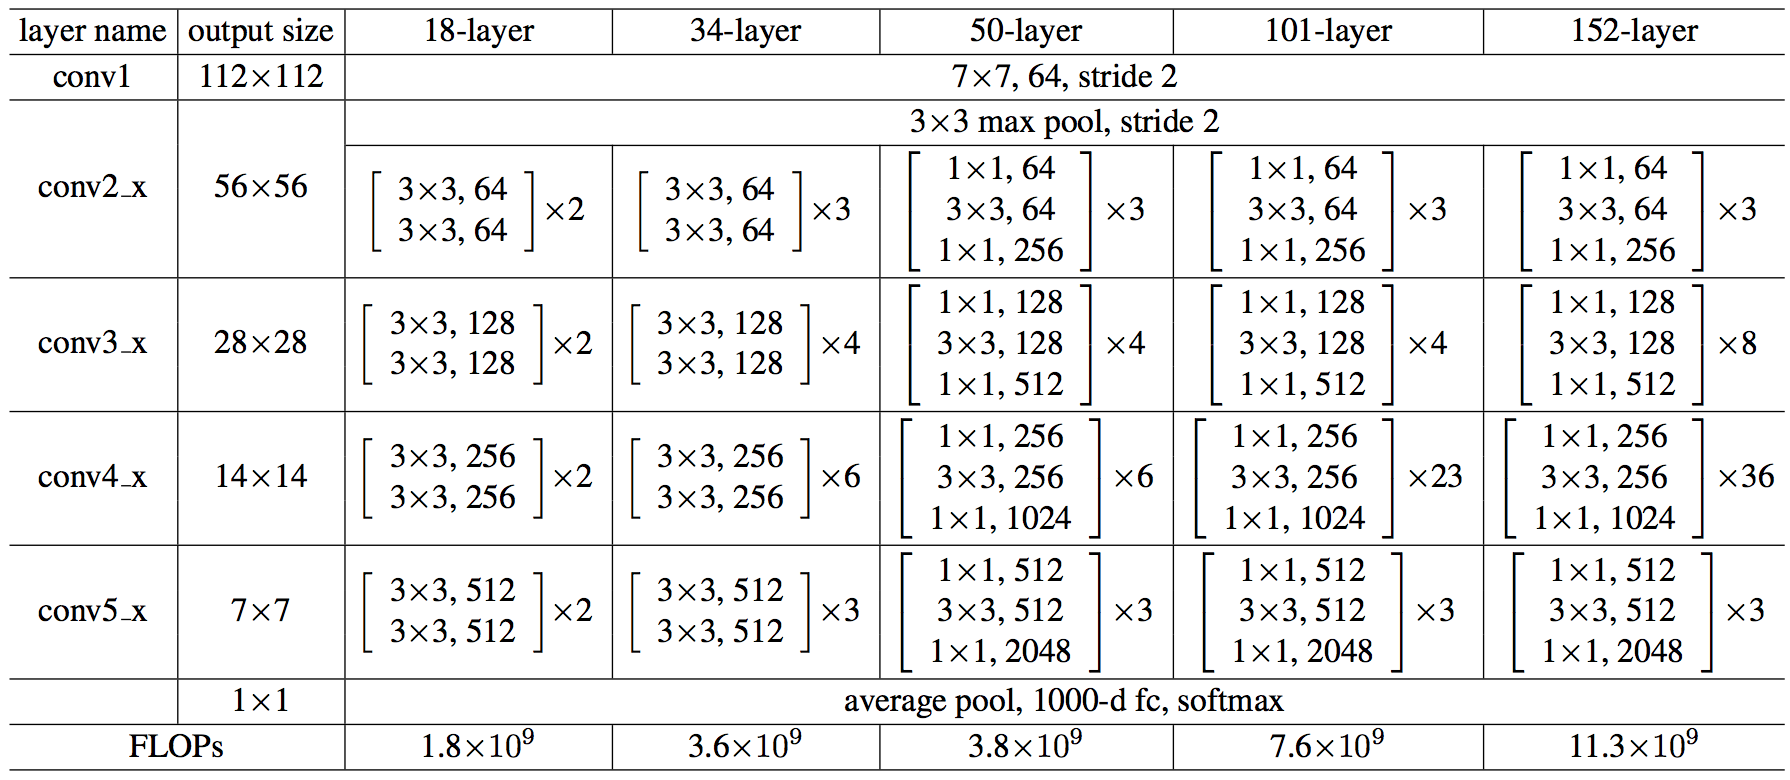
\includegraphics[width=1.0\textwidth]{fig_resnet_arch_table.png}
    \caption[Residual network architectures]{Residual network architectures for Imagenet. Building blocks are shown in brackets with the numbers of blocks stacked.}
    \caption*{Source: \href{https://neurohive.io/en/popular-networks/resnet}{https://neurohive.io/en/popular-networks/resnet}}
    \label{fig:resnet_arch_table}
    \end{center}
\end{figure}

\section{Datasets}
As most research papers evaluting \acrshort{cam}-related \acrshort{wsol} methods use the Imagenet dataset, we will use this dataset as well. Because Imagnet is a vast dataset and the our models (VGG16 and Resnet50) are computationally demanding to train, we will also use a smaller synthetic dataset. This allows us to more quickly evaluate our assumptions and implementations.

\subsection{synthetic dataset}
By using a synthetic dataset we limit computational requirements for training and evaluating our models. As we are evaluating localization of multiple object instances, using this synthetic dataset we have control over image structure, number of object instances and ground truth data. 

\subsubsection{Baseline}
For generation of the images, we took inspiration from Tjoa, E. \textit{et al.}. The authors provide algorithms for generating synthetic image datasets to quantify explainability of heatmaps in \acrshort{dnn}. The images can be generated along with the ground-truth segmentation masks for objective quantitative assessment. Each sample data is an image of a cell with easily recognized features that are  distinguished from localization ground-truth mask.
\begin{figure}[ht]
    \begin{center}       
    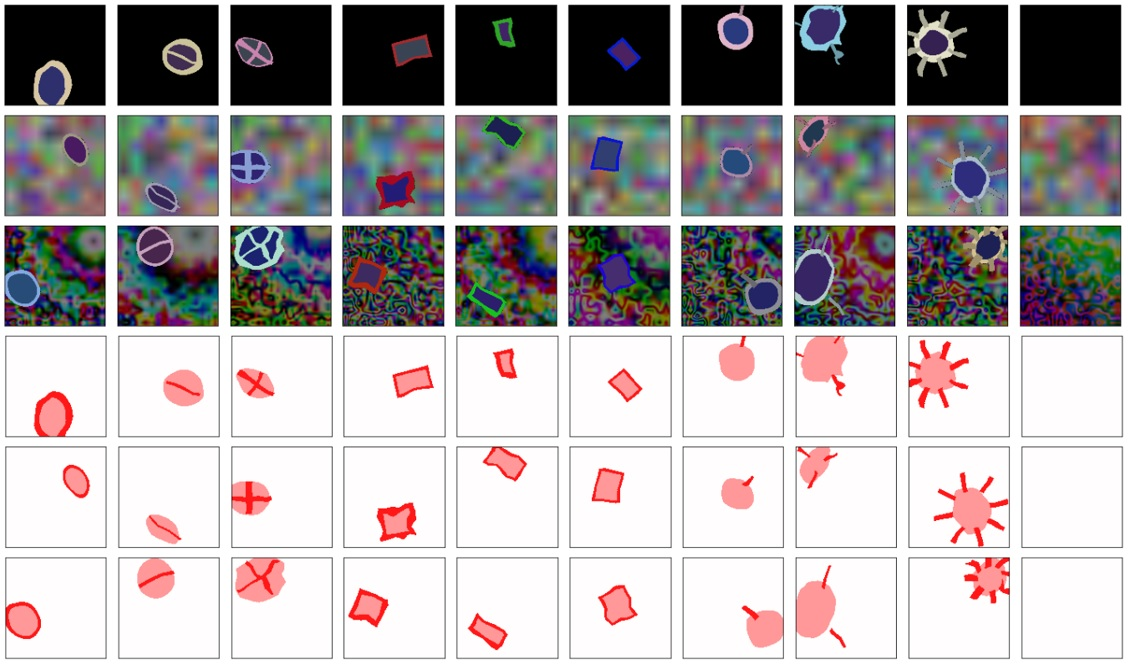
\includegraphics[width=1.0\textwidth]{fig_synthethic_paper_samples.jpeg}
    \caption[Synthetic dataset samples]{Synthetic dataset samples.}
    \caption*{Source: \href{https://github.com/ericotjo001/explainable\_ai}{https://github.com/ericotjo001/explainable\_ai}}
    \label{fig:synthetic_paper_samples}
    \end{center}
\end{figure}

Example data can be seen in Fig. \ref{fig:synthetic_paper_samples}. Ten different classes of cells are shown along the columns. Three types of backgrounds are given to increase the variation of dataset, as shown separately in the first three rows. The segmentation masks of the objects are shown in the bottom half of the figure. The classes are described in \ref{tab:synthetic_classes}.
\begin{table}[ht]
\centering
\begin{tabular}{|l|l|}
  \hline
  Class & Description \\
  \hline
  0 & Circular cell with border\\
  1 & Circular cell with minus sign\\
  2 & Circular cell with plus sign\\
  3 & Rectangular cell in red\\
  4 & Rectangular cell in green\\
  5 & Rectangular cell in blue\\
  6 & Circular cell with one tail\\
  7 & Circular cell with three tails\\
  8 & Circular cell with eight tails\\
  9 & No cell\\
  \hline
\end{tabular}
\caption[Synthetic dataset classes]{Synthetic dataset classes.}
\label{tab:synthetic_classes}
\end{table}

\subsubsection{Modifications to the baseline}
As the baseline dataset only contains single object instances, we changed the algorithms for generating images and annotations according to following criteria:
\begin{itemize}
    \item We omit class 9 as this class doesn't represent an object.
    \item We generate multiple datasets, each varying number of object instances and presence or absence of a background.
    \item Each dataset only has images with a fixed number of object instances. I.e., dataset 1 contains single-instance images, dataset 2 images only have 2 object instances, etc.
    \item All instances in an image are of the same class
    \item For each image, we create bounding box and a segmentation mask annotations to evaluate localization performance.
    \item The segmentation masks cover the full object instance region. We don't make a distinction between edge and body of an object.
\end{itemize}
We extend the baseline dataset by generating datasets with multiple object instances in the synthetic images. In addition, bounding boxes and 

\subsubsection{Datasets}
According to the criteria in previous section, we have 8 different synthetic datasets as defined in Table \ref{tab:synthetic_datasets}.
\begin{table}[ht]
\centering
\begin{tabular}{|l|l|l|l|}
  \hline
  Dataset & Instances & Background & Size\\
  \hline
  synthetic\_d1b & 1 & yes & 512x512\\
  synthetic\_d1t & 1 & no & 512x512\\
  synthetic\_d2b & 2 & yes & 512x512\\
  synthetic\_d2t & 2 & no & 512x512\\
  synthetic\_d3b & 3 & yes & 512x512\\
  synthetic\_d3t & 3 & no & 512x512\\
  synthetic\_d4b & 4 & yes & 512x512\\
  synthetic\_d4t & 4 & no & 512x512\\
  \hline
\end{tabular}
\caption[Synthetic datasets]{Synthetic datasets.}
\label{tab:synthetic_datasets}
\end{table}

Each dataset has a train, validation and test split of 1000, 200 and 200 images.

\subsection{Imagenet dataset}
We use the Imagenet dataset because it contains real, natural images with a diverse objects covering 1000 distinct classes. The dataset has multi-instance images and ground-truth image-level labels and bounding boxes. It is a very popular dataset used in many papers. It is also used in The \acrfull{ilsvrc}, a compitition that evaluates algorithms for object detection and image classification at large scale.

We use the Imagenet dataset for the classification with localization tasks as defined for the ILSVRC in 2012. The validation dataset consists of 50,000 photographs, collected from flickr and other search engines, hand labeled with the presence or absence of 1000 object categories. The training dataset is the subset of ImageNet containing the 1000 categories and 1.2 million images. The distribution of object instances over the images is show in table \ref{tab:imagenet_instance_distribution}.
\begin{table}[ht]
\centering
\begin{tabular}{rr}
\toprule
instances &  images \\
\midrule
         1 &   38285 \\
         2 &    6128 \\
         3 &    2103 \\
         4 &    1106 \\
         5 &     668 \\
         6 &     438 \\
         7 &     290 \\
         8 &     214 \\
         9 &     150 \\
        10 &     128 \\
        11 &      97 \\
        12 &      93 \\
        13 &      66 \\
        14 &      46 \\
        15 &      50 \\
        16 &      38 \\
        17 &      26 \\
        18 &      40 \\
        19 &      22 \\
        20 &      12 \\
\bottomrule
\end{tabular}
\caption[Imagenet object instance distribution]{Imagenet object instance distribution.}
\label{tab:imagenet_instance_distribution}
\end{table}

\section{Learning}
In the \acrlong{wsol} approach, we only provide image-level labels to train a model for the classification task. At test time we will provide the ground-truth labels to measure localization performance.

\begin{itemize}
    \item train classification task
    \item approach: training, tuning, pretrained datasets
    \item How we trained our models: SGD, momentum, weight decay, learning rate schedule (step, multistep), regularization (minmaxcam), model weight initialization
    \item stop criterion
\end{itemize}

% begin section to be removed
\begin{itemize}
    \item based on WSOL CAM methods
    \item learning method: Main task is classification. Localization based on learned features
    \item baseline CAM method: weighted combination of features maps with where activations are related to predicted class. Other CAM methods have specific method to compute CAM scoremap.
    \item CAM scoremap is transformed in binary scoremap using a CAM threshold = Binarized CAM scoremap is used as segmentation mask for datasets with ground truth segmentation mask labels
    \item Contours are computed in binarized CAM scoremap to derive bounding boxes for those datasets that have ground truth bounding boxes as labels. Bounding box is defined as coordinate tuple (x1, x2, y1, y2) where $x1 = x_{min}(coutour), y1 = y_{min}(contour), x2 = x_{max}(contour), y2 = y_{max}(contour)$
    \item Localization accuracy is computed by counting predicted and ground truth label matches in the evaluation dataset
\end{itemize}
% end section to be removed

\section{Localization}
To localize object instances in images, we will benchmark a set of \acrshort{cam} related methods. All those models will be evaluated using a pre-trained model on a dataset. 

 Feature activations are combined in score maps. Score maps are binarized by threshold. Contours are computed for separate components in cam map. Bounding boxes are computed and compared to ground truth during validation and test to compute localizaton metrics.

Explain selected CAM methods: reason about choice criteria, differences, benefits, limitations
CAM methods: Per cam methode: \\
- Figuur toevoegen \\
- In gewone termen uitleggen wat verschil is \\
- Formules geven en uitleggen (hoe de map gemaakt wordt) \\
Complexity computation \\
- Bezien als evaluatie methode \\
Evaluation metrics \\
- Quantitative evaluation (maxboxaccv3, pxap) \\
- Formules geven en uitleggen \\
- Complexity analysis \\

\subsection{CAM}
CAM: baseline method

\subsection{GradCAM}
GradCAM: Generalization of CAM that doesn’t require a GAP layer in the architecture

\subsection{GradCAM++}

\subsection{ScoreCAM}
ScoreCAM: Shows more focus on object instances. Also seems to do a better job in capturing the features of multiple instances in the explanation map than GradCAM.

\subsection{MinMaxCAM}
MinMaxCAM: regularization of common object regions and background

\section{Evaluation}
\subsection{Computational complexity}
Complexity computation
\begin{itemize}
    \item reasoning about choice between runtime and flops
    \item runtime cpu versus cuda (gpu), synchronization
    \item theoretical versus empirical
\end{itemize}

\subsection{Localization metrics}
\begin{itemize}
    \item Reason about existing versus required metrics
    \item Explain in detail how metrics are computed
    \item MaxBoxAccV3: modified version of MaxBoxAccV2 (Choe et al.,2020b) to support multiple instance WSOL
    \item PxAP (pixel average precision) when ground truth segmentation masks are available.
    \item explain for each method how they capture localization accuracy
    \item explain how localization of small versus large objects are affected by metrics
\end{itemize}

\section{Localization improvement}
Iterative bounding box extraction: Explain intuition for improving localization (see synthetic dataset results and how localization accuracy decreases when number of instances per images increases).

Proposal:
\begin{itemize}
    \item Feed image to model and compute feature activation maps (CAMS)
    \item Extract bounding boxes from binarized CAMS
    \item Mask bounding box areas in image (e.g. with noise, zero values)
    \item Repeat until some stop criterion
\end{itemize}
Variant: Mask image with binarized CAMs.

Possible stop criteria for iterative approach
\begin{itemize}
    \item No new bounding boxes are found
    \item Predefined drop in classification score is reached
    \item Predefined number of iterations is reached.
\end{itemize}

code references:
\begin{itemize}
    \item CAM \cite{code:CAM}
    \item MinMaxCAM \cite{code:MinMaxCAM}
    \item WSOLevaluation\cite{code:WSOLevaluation}
    \item PytorchCAM \cite{code:PytorchCAM}
\end{itemize}